\documentclass[a4paper,11pt]{article}
\usepackage{a4wide}
\usepackage{fullpage}
\usepackage[utf8x]{inputenc}

\usepackage[light,math]{anttor}
\usepackage[T1]{fontenc}

%\usepackage[slovene]{babel}
%\selectlanguage{slovene}
\usepackage[toc,page]{appendix}
\usepackage[pdftex]{graphicx} 

\usepackage{lmodern}
\usepackage{amsmath}
\usepackage{amssymb}
\usepackage{amsthm}
\usepackage{amsfonts}
\usepackage{mathtools}
\usepackage{enumitem}
\usepackage{amsfonts}
\usepackage{amsmath}
\usepackage{setspace}
\usepackage{color}
\definecolor{light-gray}{gray}{0.95}
\usepackage{listings} 
\usepackage{hyperref}

\renewcommand{\baselinestretch}{1.2} 
\renewcommand{\appendixpagename}{Priloge}


\title{Bayesova statistika: Domača naloga 2 }
\author{Sara Bizjak  |  27202020}
\date{December 2021}

%%%%%%%%%%%%%%%%%%%%%%%%%%%%%%%%%%%%%%%%%%%%%%%%%%%%%%%%%%%%%%%%%%%%%%%%%%%%%%%%%%%%%%%%%%%%%%%%%%%%%%%%%%%%%%%%%%%%%%%%%%%%%%%%%

\begin{document}

\maketitle
\noindent
Implementacija algoritma je dostopna v priloženi datoteki \texttt{DN2\_koda\_sarabizjak.R}. Prav tako so v tej datoteki zapisani klici, s pomočljo katerih sem dobila vse spodnje grafe in rezultate.
\\
\\
\noindent
\textbf{1. naloga: Implementacija algoritma Metropolis-Hastings}
\\
Za predlagalno jedro smo izbrali 
\begin{align*}\label{predlagalno_jedro}
    \sigma_q = 0.1
\end{align*}
Privzamemo normalni model, kjer 
$$(X_i | \theta) \sim N( \theta, \sigma^2 = 4),$$
kjer ocenjujemo porazdelitev $\theta$, 
apriorna porazdelitev pa je 
$$\theta \sim N(\theta_0 = 6, \tau_0^2 = 9)$$
Zanima nas aposteriorna porazdelitev $(\theta | X)$, ki je porazdeljena normalno $N( \theta_1, \tau_1^2)$, kjer sta parametra enaka
\begin{align*} 
    \theta_1 &= \frac{\tau_0^2}{\frac{\sigma^2}{n} + \tau_0^2} \ \overline{X} + \frac{\frac{\sigma^2}{n}}{\frac{\sigma^2}{n} + \tau_0^2} \ \theta_0
    \\
    \tau_1^2 &= \frac{\frac{\sigma^2}{n} \cdot \tau_0^2}{\frac{\sigma^2}{n} + \tau_0^2}
\end{align*}

\noindent
\textbf{2. naloga: Smiselna začetna vrednost}
\\
Preizkus algoritma na primeru, kjer so podatki število ur, ki so jih dijaki potrebovali za pripravo domače naloge:
\begin{align*} 
    x = [2.11, 9.75, 13.88, 11.3, 8.93, 15.66, 16.38, 4.54, 8.86, 11.94, 12.47, 11.11, 
    \\
    11.65, 14.53, 9.61, 7.38, 3.34, 9.06, 9.45, 5.98, 7.44, 8.5, 1.55, 11.45, 9.73]
\end{align*}
Smiselno začetno vrednost lahko interpretiramo kot izbor kateregakoli naravnega števila, ki ni preveliko, torej število ur, ki je smiselno za izdelavo domače naloge.
Za začetno vrednost bi torej lahko vzeli denimo število 5. V Bayesovi statistiki pa za začetno vrednost v takem primeru v praksi (ponavadi) vzamemo kar število blizu povprečja ali povprečje samo. 
Ker je $mean(x) = 9.464$, je tukaj potem smiselna izbira začetne vrednosti 9. Da vidimo razliko, si poglejmo obe varianti.
Za celotno zaporedje bomo vzeli $100000$ iteracij.

\noindent
\textbf{Izrisano celotno dobljeno zaporedje.}
    \begin{figure}[ht!]
        \begin{minipage}{0.5\textwidth}
            \centering
            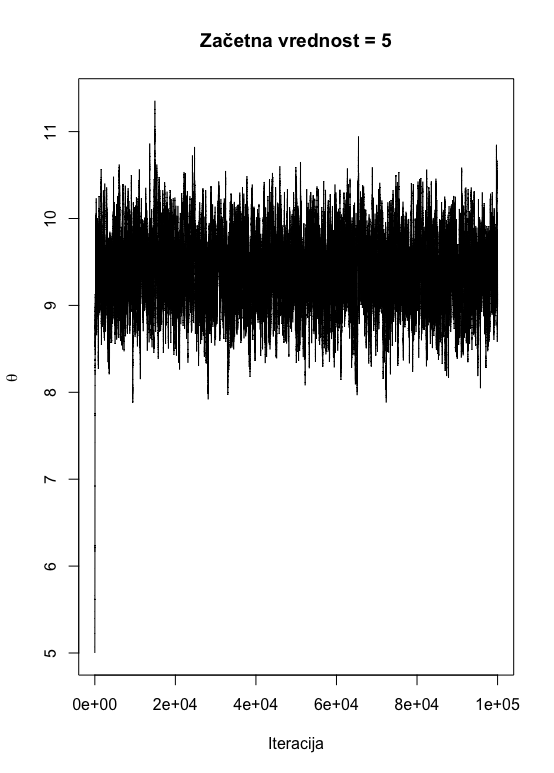
\includegraphics[width = 60mm]{Slike/2_1_zv5.png}
            \caption{Celotno zaporedje, zv = 5.}
        \end{minipage}
        \begin{minipage}{0.5\textwidth}
            \centering
            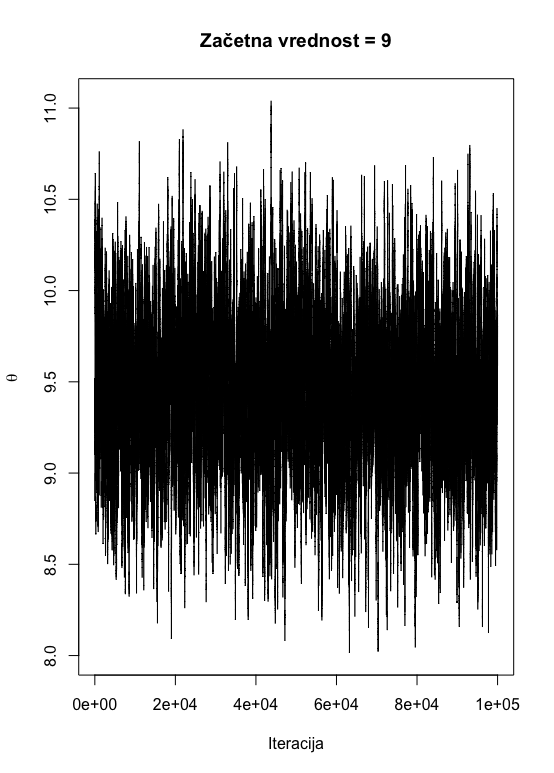
\includegraphics[width = 60mm]{Slike/2_1_zv9.png}
            \caption{Celotno zaporedje, zv = 9.}
        \end{minipage}
    \end{figure}

    \noindent
\textbf{Izrisanih prvih 500 in prvih 5000 členov.}
    \begin{figure}[ht!]
        \begin{minipage}{0.5\textwidth}
            \centering
            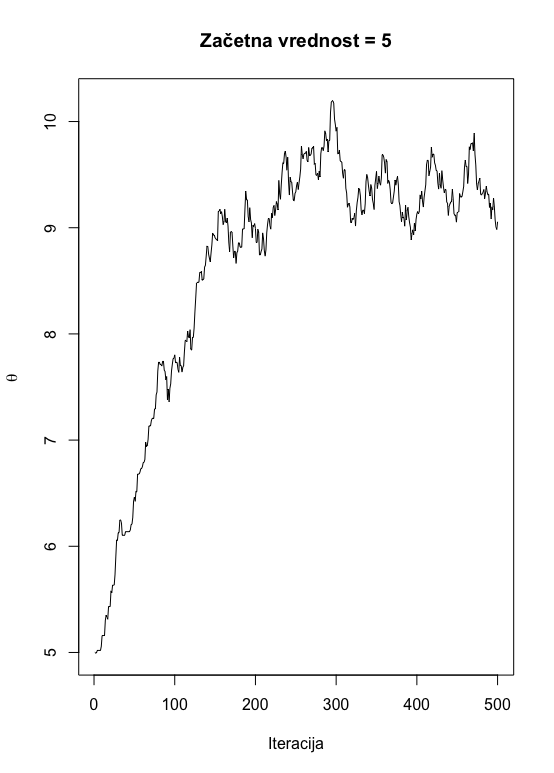
\includegraphics[width = 65mm]{Slike/2_2_500_zv5.png}
            \caption{$500$ iteracij, zv = 5.}
        \end{minipage}
        \begin{minipage}{0.5\textwidth}
            \centering
            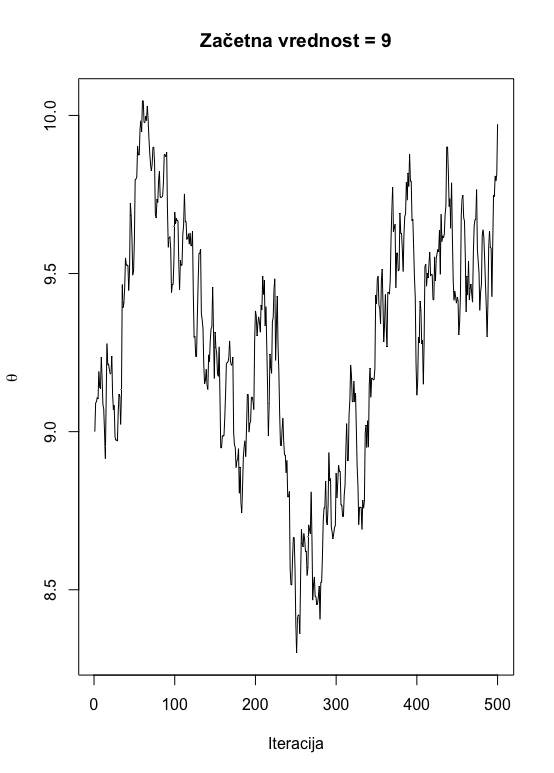
\includegraphics[width = 65mm]{Slike/2_2_500_zv9.png}
            \caption{$500$ iteracij, zv = 9.}
        \end{minipage}
    \end{figure}
    \begin{figure}[ht!]
        \begin{minipage}{0.5\textwidth}
            \centering
            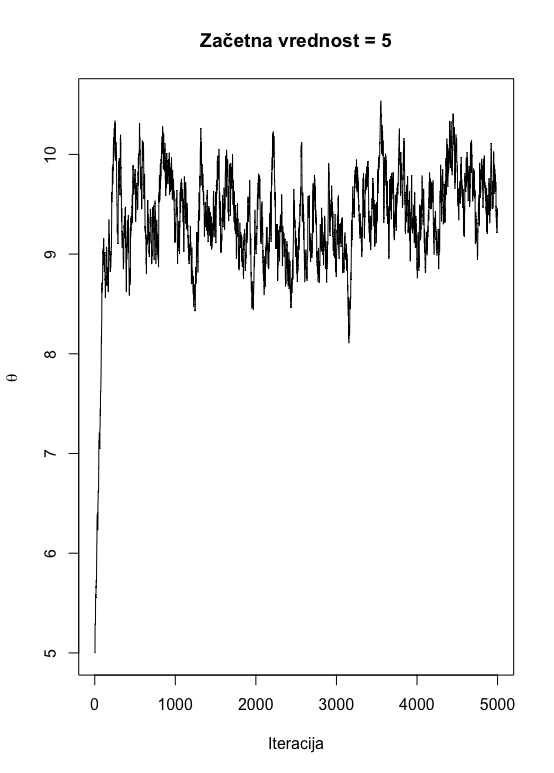
\includegraphics[width = 65mm]{Slike/2_2_5000_zv5.png}
            \caption{$5000$ iteracij, zv = 5.}
        \end{minipage}
        \begin{minipage}{0.5\textwidth}
            \centering
            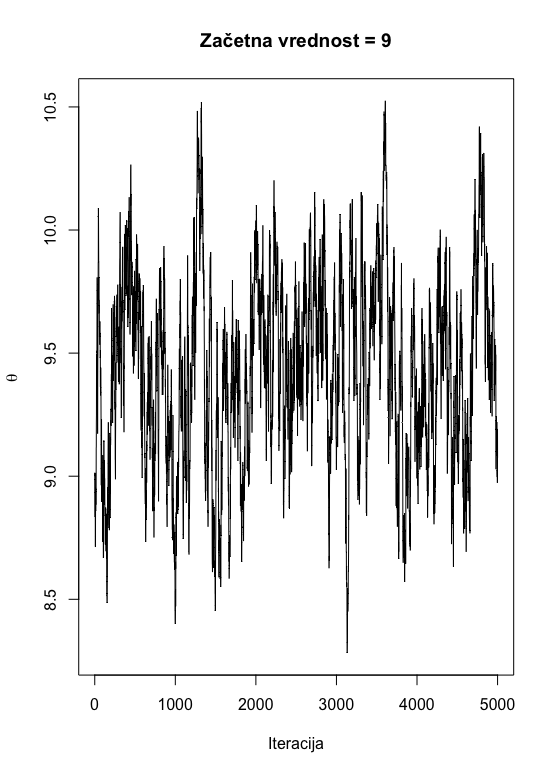
\includegraphics[width = 65mm]{Slike/2_2_5000_zv9.png}
            \caption{$5000$ iteracij, zv = 9.}
        \end{minipage}
    \end{figure}

\noindent
Hitro opazimo, da konvergenca pri začetni vrednosti 5 potrebuje več časa, to pomeni, da je potrebnih več iteracij, da se vrednost "stabilizira okrog povprečja" oz. se začne gibati po nekem območju (gor in dol).
Pri začetni vrednosti 9 pa so vrednosti že na začetku v želem območju, tako da je zaporedje od prve iteracije pa do konca v tem območju.
Omenimo še, da je tukaj "gibanje/stabilizacija okoli povprečja" mišljeno kot gibanje v območju aposteriorne porazdelitve.
\\
Izbira burn-in parametra je torej odvisna od konkretne začetne vrednosti -- drugače bi izbrali za vrednosti 5 in 9, pa tudi, če sta obe smiselni za naš primer.
\\ 
Pri začetni vrednosti 5 bi za burn-in parameter lahko izbrali $B = 500$, pri začetni vrednosti 9 pa je zaporedje dovolj stabilno že od samega začetka, tako da bi lahko za nadaljevanje opazovali vse vrednosti, to pomeni, da bi burn-in parameter verjetno lahko nastavili na 0. 
Ker pa ponavadi izberemo $B > 0$ -- sploh za kompleksnejše modele -- bi za $B$ določili neko manjšo vrednost, da bi se še vseeno izognili morebitnim začetnim "kalibracijam", recimo $B = 100$.
\\
V nadaljevanju bodo vse smiselne začetne vrednosti nastavljene na $5$, tako da bo konvergenca (pa tudi burn-in parameter) bolj izrazita. Podobni zaključki pa bi veljali tudi za izbiro $zv = 9$.
\\

\newpage
\noindent
\textbf{Izrisano celotno dobljeno zaporedje z burn-in parametrom B = 500.}
    \begin{figure}[ht!]
        \centering
        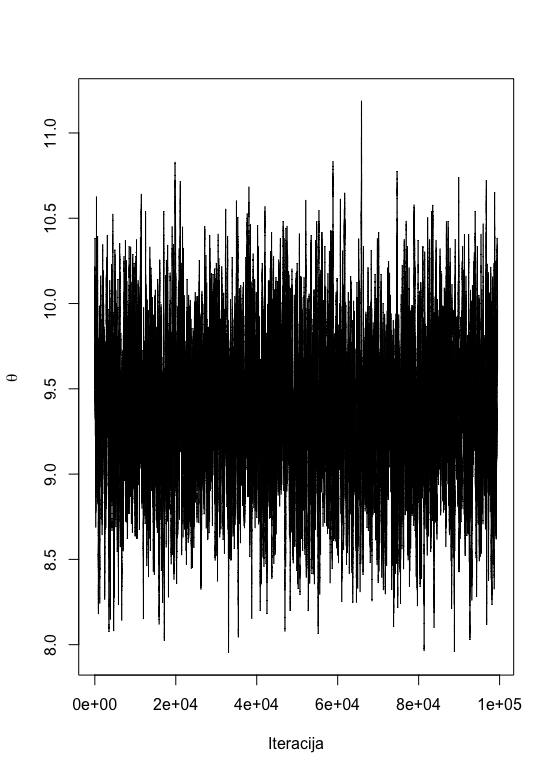
\includegraphics[width = 65mm]{Slike/2_3.png}
        \caption{Celotno zaporedje z burn-in parametrom $B = 500$.}
    \end{figure}

\noindent
\textbf{Grafična primerjava teoretične aposteriorne porazdelitve in dobljene z algoritmom M-H.}
    \begin{figure}[ht!]
            \centering
            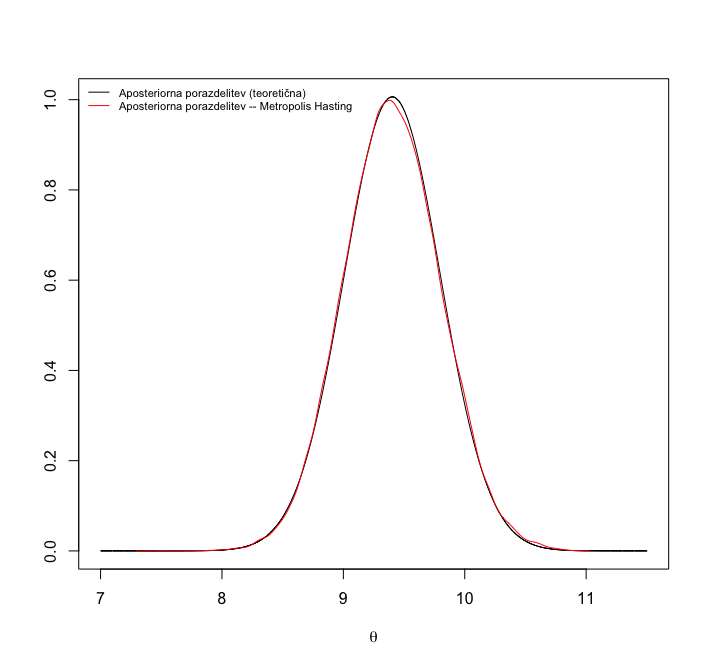
\includegraphics[width = 110mm]{Slike/2_4a.png}
            \caption{Primerjava aposteriornih porazdelitev (ob upoštevanju burn-in parametra).}
    \end{figure}

\newpage
\noindent
\textbf{Primerjava 95\% intervala zaupanja teoretične aposteriorne porazdelitve in dobljene z algoritmom Metropolis Hastings.}
\\
\noindent
95\% intervala zaupanja teoretične aposteriorne porazdelitve: 
\\
\texttt{[8.626385     10.180602]}
\\[0.1cm]
95\% intervala zaupanja porazdelitve dobljene z Metropolis Hastings:
\\
\texttt{[8.628473    10.187521]}
\\
\\
\noindent
\textbf{3. naloga: Nesmiselna začetna vrednost}
\\
Za nesmiselno začetno vrednost izberemo vrednost -1. Vrednost -1 je res nesmiselna, saj podani vektor vsebuje število ur, ki so jih učenci porabili za izdelavo domačih nalog, za to dejanje pa je nemogoče porabiti -1 uro.

\noindent
\textbf{Izrisano celotno dobljeno zaporedje.}
    \begin{figure}[ht!]
        \centering
        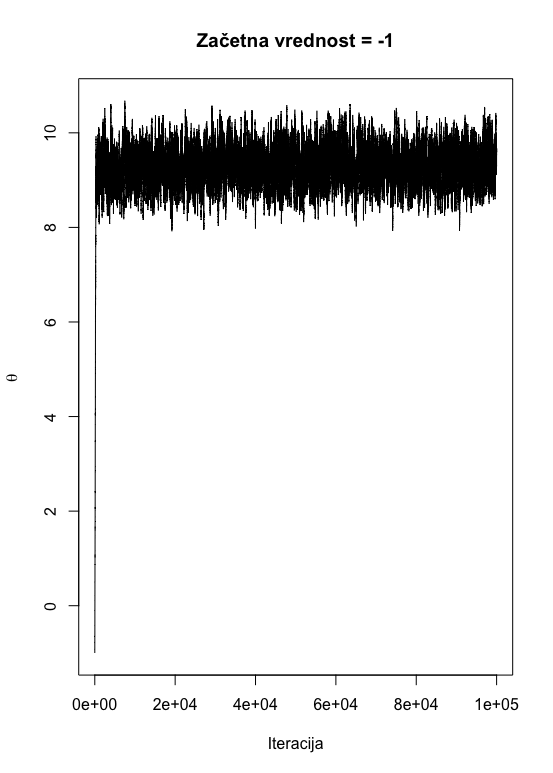
\includegraphics[width = 65mm]{Slike/3_1.png}
        \caption{Celotno zaporedje, zv = -1.}
    \end{figure}
\newpage
\noindent
\textbf{Izrisanih prvih 500 in prvih 5000 členov.}
    \begin{figure}[ht!]
        \begin{minipage}{0.5\textwidth}
            \centering
            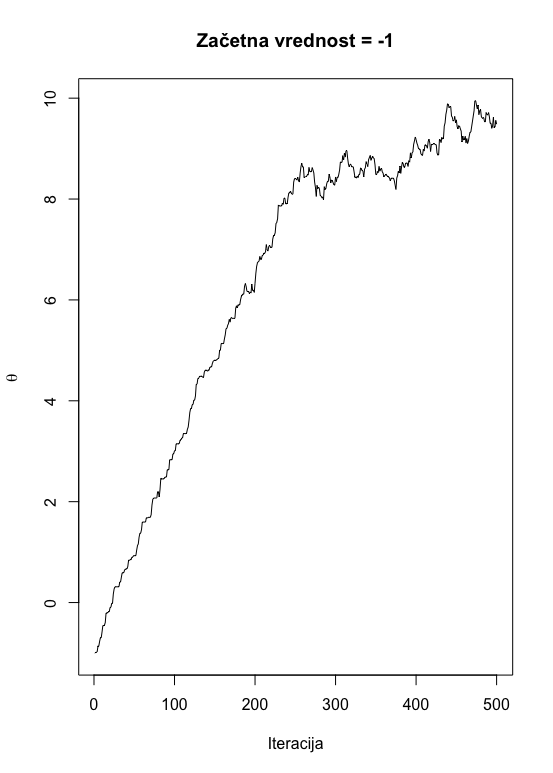
\includegraphics[width = 55mm]{Slike/3_2.png}
            \caption{$500$ iteracij, zv = -1.}
        \end{minipage}
        \begin{minipage}{0.5\textwidth}
            \centering
            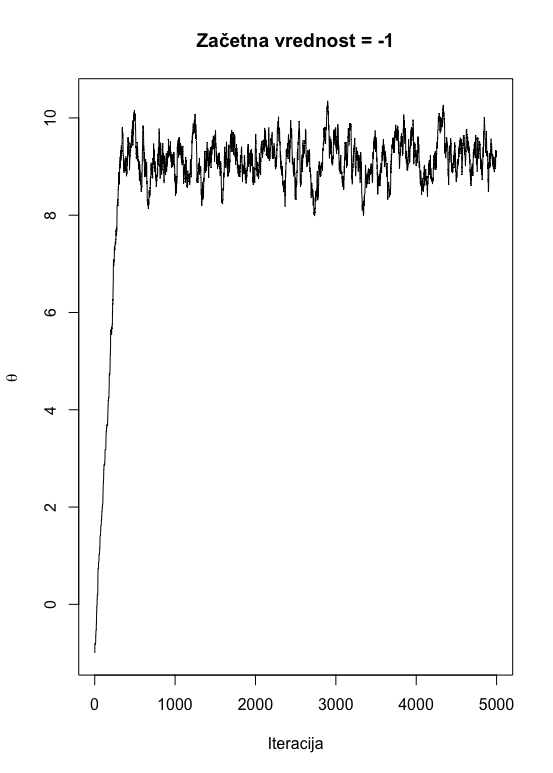
\includegraphics[width = 55mm]{Slike/3_2_5000.png}
            \caption{$5000$ iteracij, zv = -1.}
        \end{minipage}
    \end{figure}

\noindent
Ker je tokrat izbrana začetna vrednost nesmiselna, kar hkrati pomeni, da je izbrana daleč od povprečja, je konvergenca bolj počasna kot pri smiselno izbrani vrednosti. To pomeni, da je potrebnih več iteracij, da se veriga začne gibati v območju aposteriorne porazdelitve.
Zato je temu primerna tudi izbira burn-in parametra, ki mora biti v tem primeru večji.

\noindent
\textbf{Izrisano celotno dobljeno zaporedje z burn-in parametrom B = 1000.}
    \begin{figure}[ht!]
        \centering
        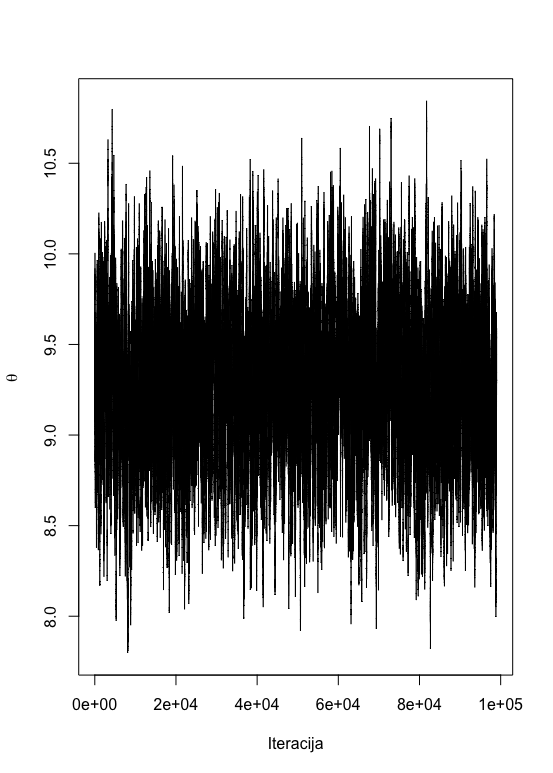
\includegraphics[width = 65mm]{Slike/3_3.png}
        \caption{Celotno zaporedje z burn-in parametrom $B = 1000$.}
    \end{figure}



\newpage
\noindent
\textbf{4. naloga: Kalibracija variance predlagalnega jedra}
\\
\noindent
Izrišimo prvih 5000 členov in celotno zaporedje za različne variance predlagalnega jedra ob smiselni začetni vrednosti 5 kot v prejšnjih primerih.  

    \begin{figure}[ht!]
        \begin{minipage}{0.5\textwidth}
            \centering
            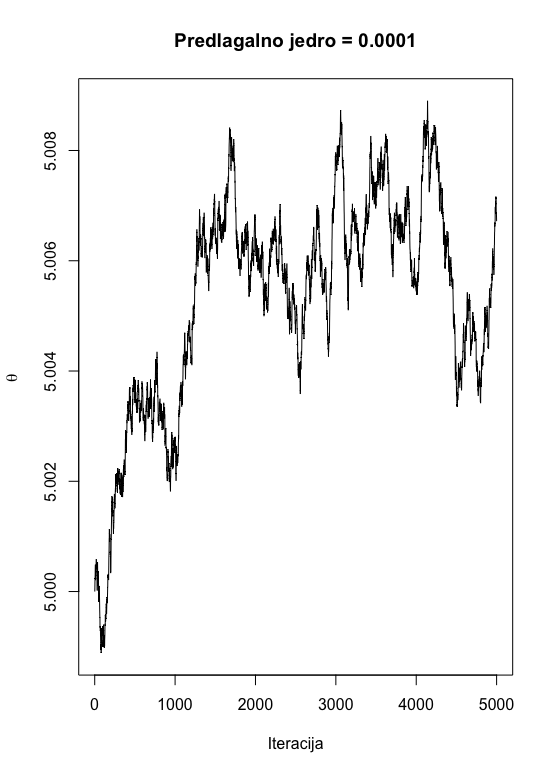
\includegraphics[width = 60mm]{Slike/4_1a_S.png}
            \caption{Prvih 5000 členov.}
        \end{minipage}
        \begin{minipage}{0.5\textwidth}
            \centering
            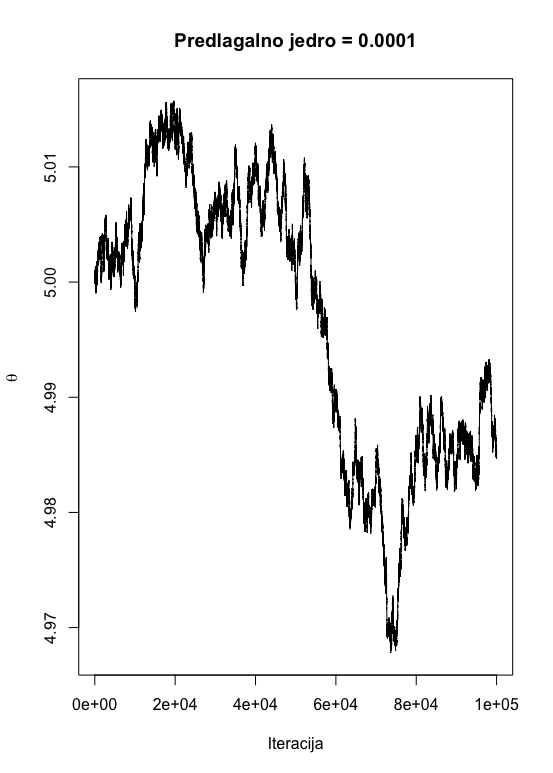
\includegraphics[width = 60mm]{Slike/4_1a_celotno.png}
            \caption{Celotno zaporedje.}
        \end{minipage}
    \end{figure}

    \begin{figure}[ht!]
        \begin{minipage}{0.5\textwidth}
            \centering
            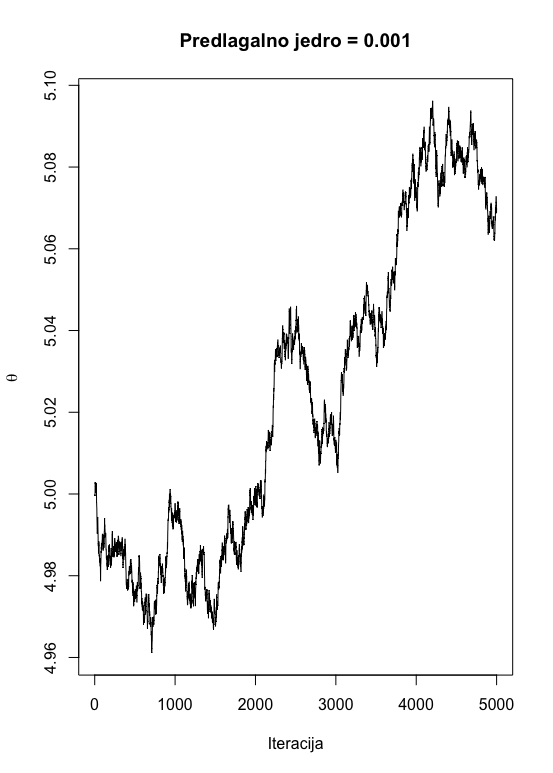
\includegraphics[width = 60mm]{Slike/4_1b_S.png}
            \caption{Prvih 5000 členov.}
        \end{minipage}
        \begin{minipage}{0.5\textwidth}
            \centering
            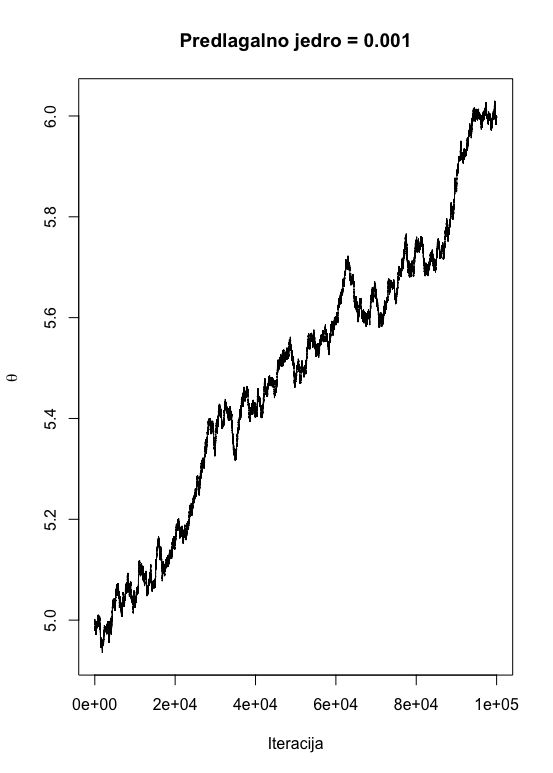
\includegraphics[width = 60mm]{Slike/4_1b_celotno.png}
            \caption{Celotno zaporedje.}
        \end{minipage}
    \end{figure}
\newpage
    \begin{figure}[ht!]
        \begin{minipage}{0.5\textwidth}
            \centering
            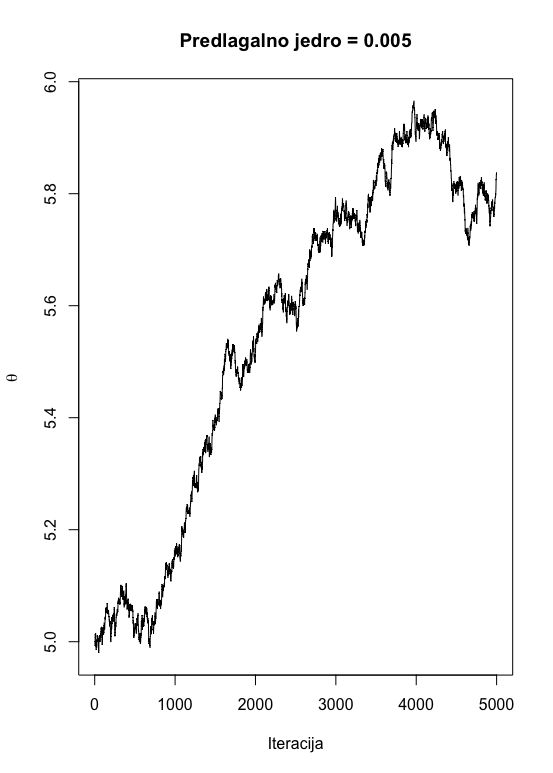
\includegraphics[width = 60mm]{Slike/4_1c_S.png}
            \caption{Prvih 5000 členov.}
        \end{minipage}
        \begin{minipage}{0.5\textwidth}
            \centering
            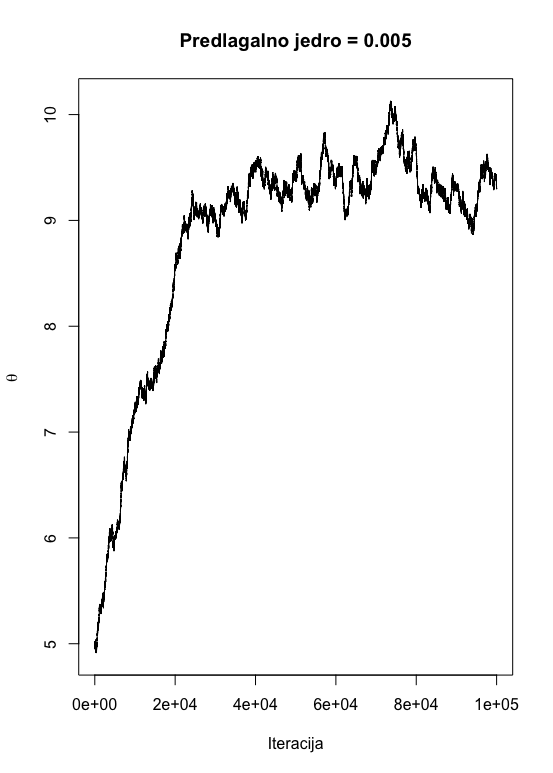
\includegraphics[width = 60mm]{Slike/4_1c_celotno.png}
            \caption{Celotno zaporedje.}
        \end{minipage}
    \end{figure}

    \begin{figure}[ht!]
        \begin{minipage}{0.5\textwidth}
            \centering
            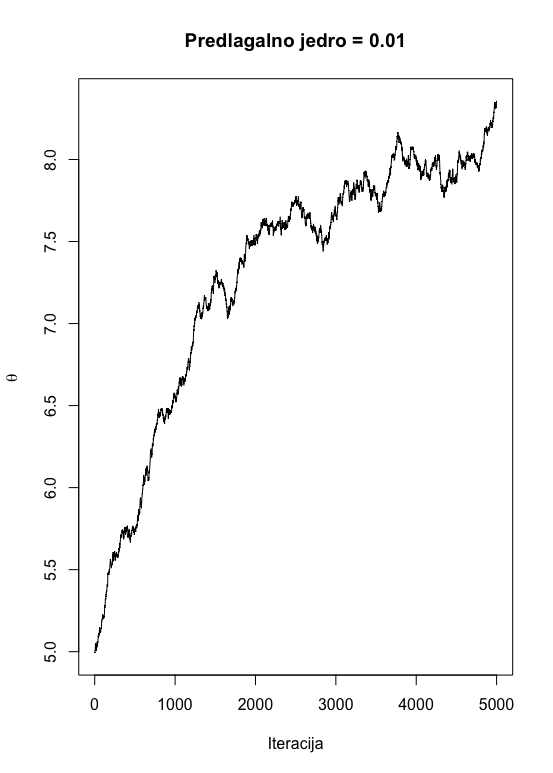
\includegraphics[width = 60mm]{Slike/4dod_S.png}
            \caption{Prvih 5000 členov.}
        \end{minipage}
        \begin{minipage}{0.5\textwidth}
            \centering
            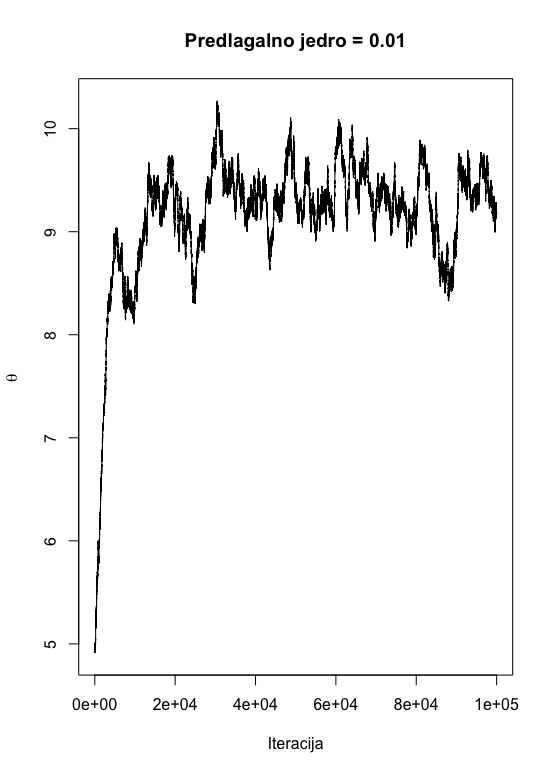
\includegraphics[width = 60mm]{Slike/4dod_celotno.png}
            \caption{Celotno zaporedje.}
        \end{minipage}
    \end{figure}
\newpage
    \begin{figure}[ht!]
        \begin{minipage}{0.5\textwidth}
            \centering
            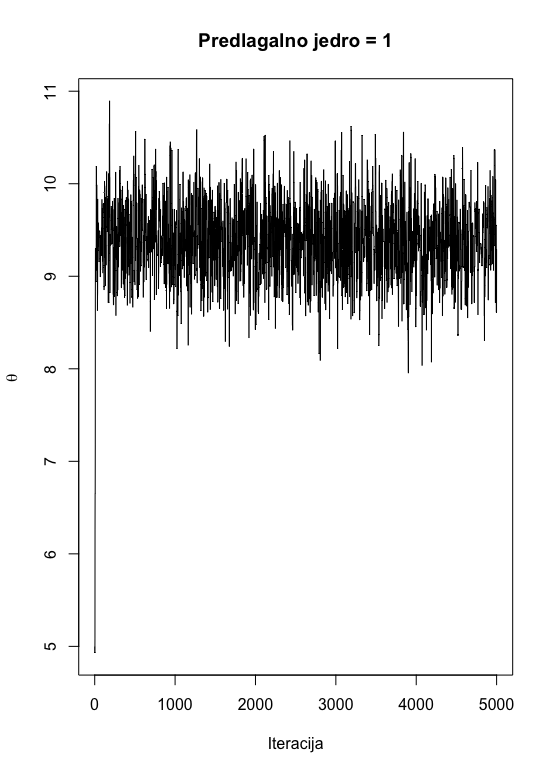
\includegraphics[width = 60mm]{Slike/4_1d_S_s.png}
            \caption{Prvih 5000 členov.}
        \end{minipage}
        \begin{minipage}{0.5\textwidth}
            \centering
            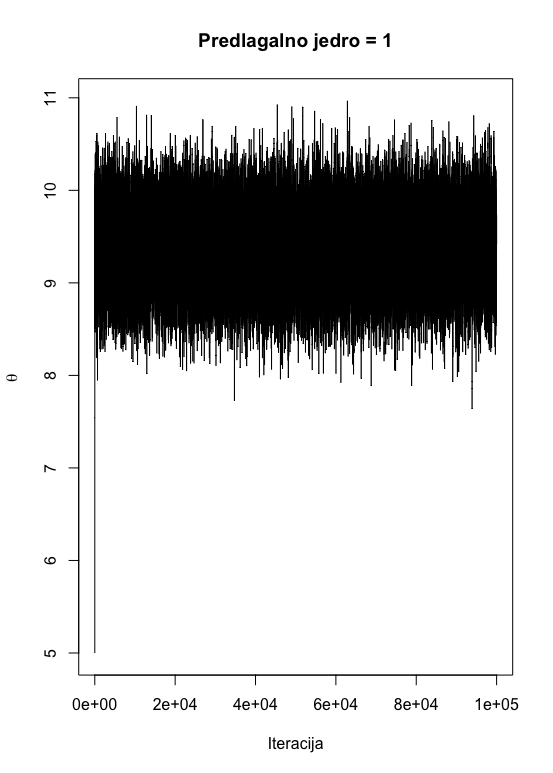
\includegraphics[width = 60mm]{Slike/4_ad_celotno_s.png}
            \caption{Celotno zaporedje.}
        \end{minipage}
    \end{figure}

    \begin{figure}[ht!]
        \begin{minipage}{0.5\textwidth}
            \centering
            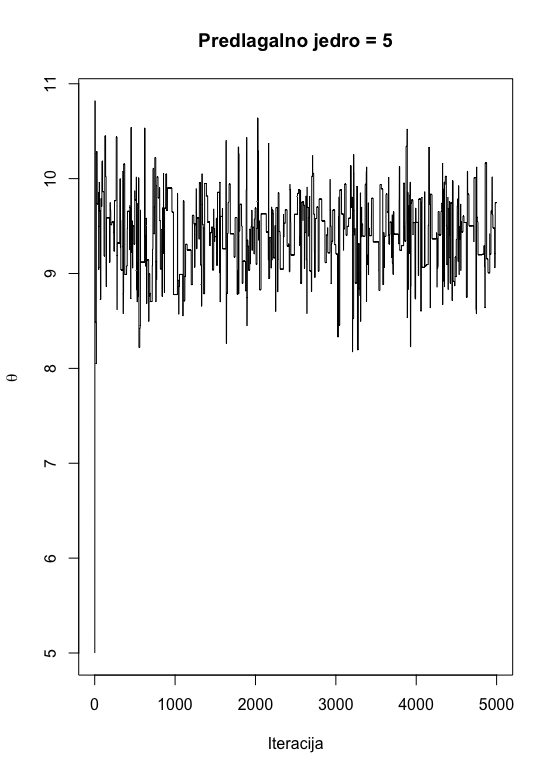
\includegraphics[width = 60mm]{Slike/4_1e_S_s.png}
            \caption{Prvih 5000 členov.}
        \end{minipage}
        \begin{minipage}{0.5\textwidth}
            \centering
            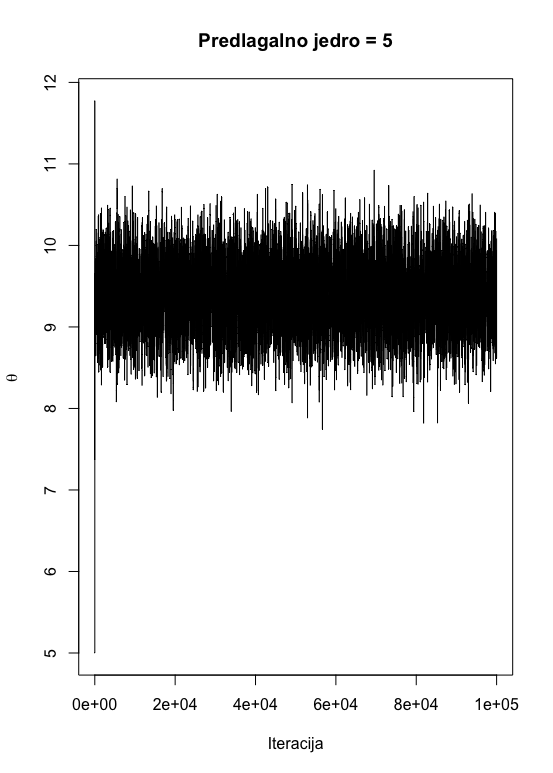
\includegraphics[width = 60mm]{Slike/4_1e_celotno_s.png}
            \caption{Celotno zaporedje.}
        \end{minipage}
    \end{figure}
\newpage
    \begin{figure}[ht!]
        \begin{minipage}{0.5\textwidth}
            \centering
            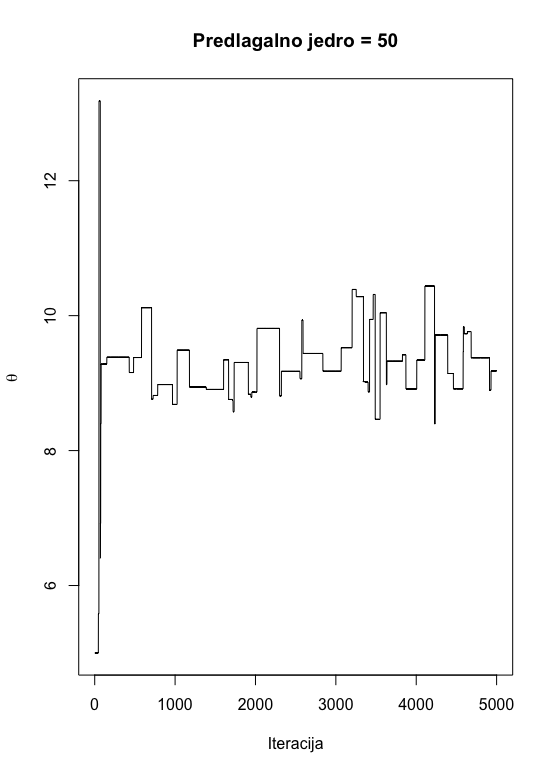
\includegraphics[width = 60mm]{Slike/4_1f_S_s.png}
            \caption{Prvih 5000 členov.}
        \end{minipage}
        \begin{minipage}{0.5\textwidth}
            \centering
            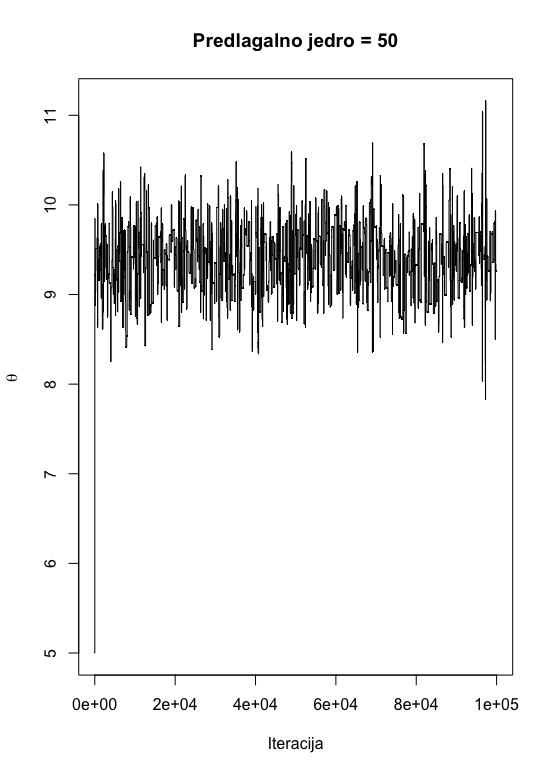
\includegraphics[width = 60mm]{Slike/4_1f_celotno_s.png}
            \caption{Celotno zaporedje.}
        \end{minipage}
    \end{figure}


\noindent
Najprej komentirajmo, da če bi enake grafe izrisali pri predlagalnem jedru $\sigma_q = -1$ bi v splošnem dobili počasnejše konvergence, podobno kot smo opazili že zgoraj.
\\
\\
Za zelo majhna predlagalna jedra vidimo, da zaporedje v $100000$ korakih (naše celotno zaporedje) ne skonvergira. Prva dokončna konvergenca se opazi šele pri izbira jedra $\sigma_q = 0.005$, ampak je konvergenca zelo počasna.
\\
Lahko rečemo, da v splošnem velja, da večje predlagalno jedro privede do hitrejše konvergence, kar pa ni vedno najboljše. 
Če za $\sigma_q$ izbiramo vrednosti, ki so večje od tiste, ki smo jo uporabili kot privzeto v našem algoritmu ($\sigma_q > 0.1$), opazimo, da je konvergenca sicer zelo hitra, a se na grafih zaporedij pojavljajo stopničke (še bolje bi se videlo na grafu z manj iteracijami), kar pomeni, da je naslednji člen velikokrat enak prejšnjemu in je veliko posameznih delov zaporedja konstantnih.
In večja kot je $\sigma_q$, daljše so te stopničke oz. je veriga čez vedno več iteracij konstanta.
\\
Če torej simuliramo porazdelitev slučajne spremenljivke z neustrezno izbranim predlagalnim jedrom (v kombinaciji z neustrezno izbrano začetno vrednostjo), je porazdelitev neustrezna in algoritem v takem primeru ne vrne željenega rezultata.
\\
\\
Izbira variance predlagalnega jedra je verjetno odvisna od situacije oz. zastavljenega problema. Odvisno je seveda tudi od tega, kaj želimo z izračunom doseči.
V splošnem pa opazimo dve skrajnosti: 
\begin{itemize}
    \item vrednost $\sigma_q$ (pre)majhna: konvergenca je počasna, a s členi zaporedja območje aposteriorne porazdelitve dobro raziščemo -- raziskujemo počasi, delamo majhne korake, vendar ne delamo "stopničk" (tej situaciji rečemo \textit{too high acceptance rate}),
    \item vrednost $\sigma_q$ (pre)velika: konvergenca je hitra, zaporedje se v zelo hitrem času začne gibati po območju aposteriorne porazdelitve, ne razišče pa je (dovolj) dobro (imamo "stopničke") (tej situaciji rečemo \textit{too low acceptance rate}).
\end{itemize}
Kot smo videli nobena skrajnost ni dobra, zato bi predlagala, da v splošnem iščemo kompromis med tema dvema možnostima.
Za naš primer velja, da je $\sigma_q$ za stopnjo $10^1$ manjša od $\sigma$ privzetega modela. To pa ne nujno velja tudi v splošnem.
\\
Menim, da bi najbolj splošen pristop bil, da bi definirali test, ki bi ocenil, ali je ob izbranem $\sigma_q$ konvergenca dobra (po zgornjih standardih, torej da se ne zgodi nobena situacija iz zgornjih alinej).
To bi lahko naredili na več načinov.
\\
En tak test bi denimo lahko bil Gelman-Rubin test konvergence, ki ga poženemo na več simuliranih verigah. Tako bi lahko izbrali nekaj vrednosti za $\sigma_q$ in ugotovili, katera izbira je najboljša (ob predpostavki, da bi za začetno vrednost vedno izbrali vrednost blizu povprečja).
\\
Podoben test za oceno konvergence bi (verjetno) lahko uporabili tudi vzporedno z uporabo nekakšnega meta učenja (strojno učenje). To bi naredili tako, da bi najboljšo izbiro za $\sigma_q$ izbrali s preiskovanjem prostora parametrov. Torej najprej bi algoritem določil ustrezno vrednost za $\sigma_q$, potem pa bi s to vrednostjo za $\sigma_q$ naredili ustrezne simulacije.
\\
Lahko pa bi ubrali tudi adaptiven pristop, ki bi na vsakih $N$ iteracij izračunal delež sprejetih novih členov (takih, ki niso enaki prejšnjim, da ne delamo stopničk). Glede na izračunan delež bi potem prilagodili $\sigma_q$ (povečali ali pomanjšali).
\\
Zasledila sem tudi pristop redčenja verig (\textit{thinning}), ki pa se v praksi opušča, saj je končni vzorec bistveno manjši od vseh "pregledanih" členov, saj v končno porazdelitev izberemo le vsak $k$-ti člen in zato jih veliko izpustimo.


\end{document}

\begin{thebibliography}{99}

\end{thebibliography}





\newpage
\noindent
\textbf{(b) začetna vrednost = -1.}
    \begin{figure}[ht!]
        \begin{minipage}{0.5\textwidth}
            \centering
            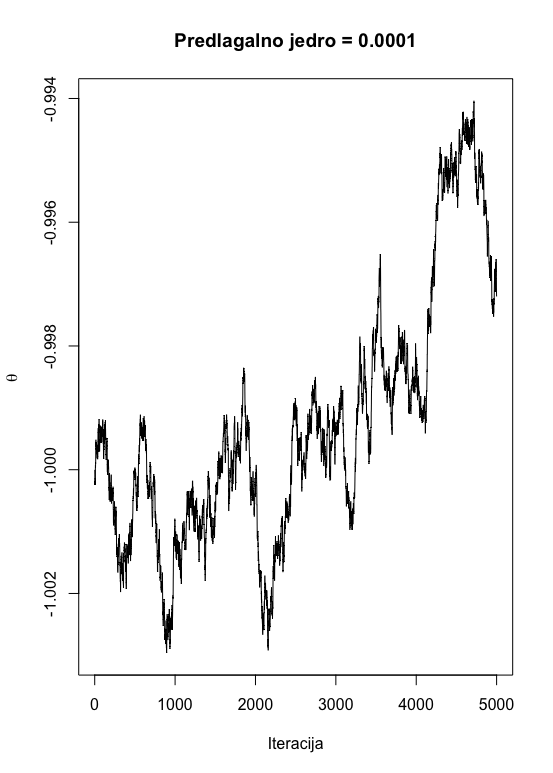
\includegraphics[width = 60mm]{Slike/4_1a_S_ne.png}
            \caption{Prvih 5000 členov.}
        \end{minipage}
        \begin{minipage}{0.5\textwidth}
            \centering
            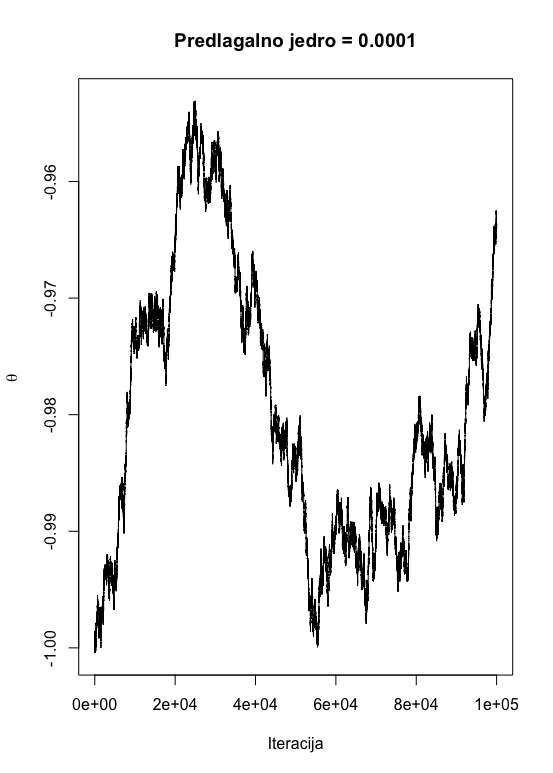
\includegraphics[width = 60mm]{Slike/4_1a_celotno_ne.png}
            \caption{Celotno zaporedje.}
        \end{minipage}
    \end{figure}

    \begin{figure}[ht!]
        \begin{minipage}{0.5\textwidth}
            \centering
            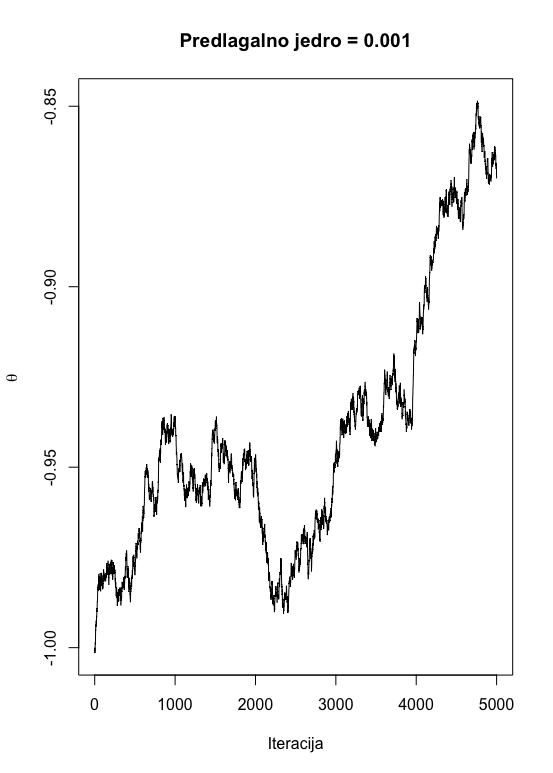
\includegraphics[width = 60mm]{Slike/4_1b_S_ne.png}
            \caption{Prvih 5000 členov.}
        \end{minipage}
        \begin{minipage}{0.5\textwidth}
            \centering
            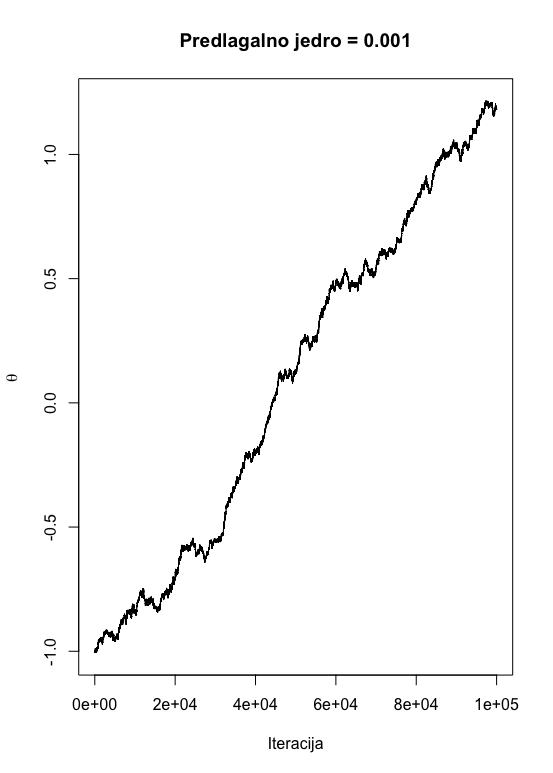
\includegraphics[width = 60mm]{Slike/4_1b_celotno_ne.png}
            \caption{Celotno zaporedje.}
        \end{minipage}
    \end{figure}

    \begin{figure}[ht!]
        \begin{minipage}{0.5\textwidth}
            \centering
            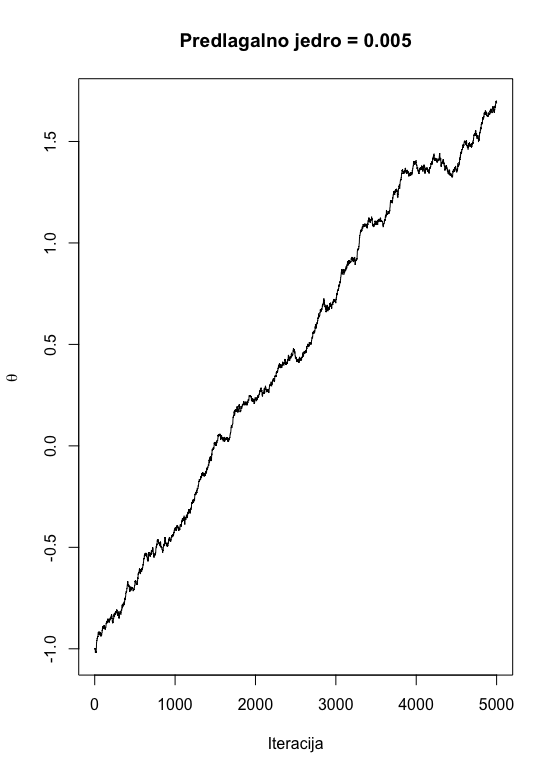
\includegraphics[width = 60mm]{Slike/4_1c_S_ne.png}
            \caption{Prvih 5000 členov.}
        \end{minipage}
        \begin{minipage}{0.5\textwidth}
            \centering
            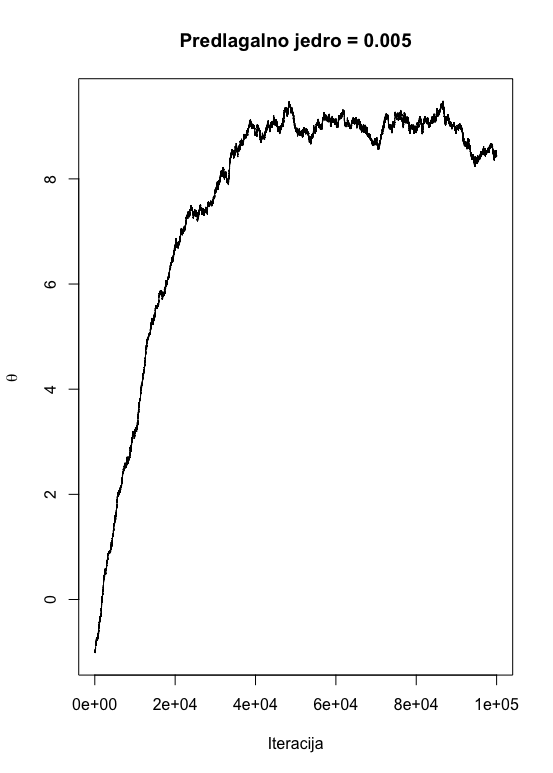
\includegraphics[width = 60mm]{Slike/4_1c_celotno_ne.png}
            \caption{Celotno zaporedje.}
        \end{minipage}
    \end{figure}

    \begin{figure}[ht!]
        \begin{minipage}{0.5\textwidth}
            \centering
            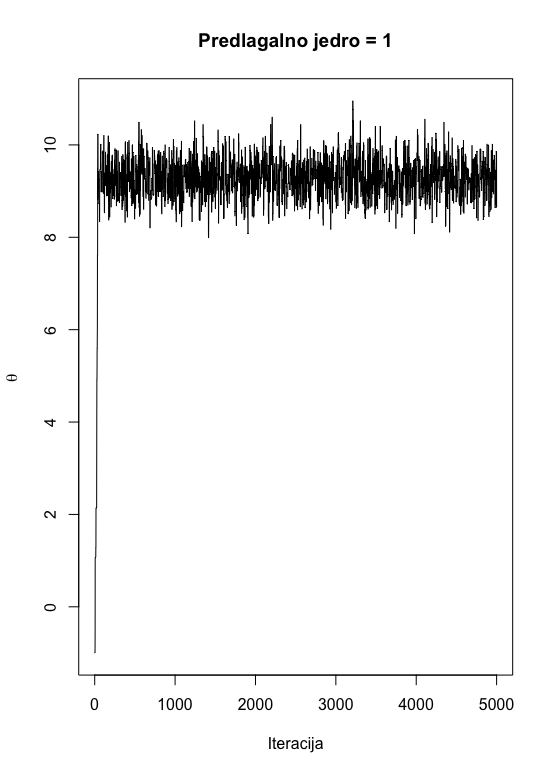
\includegraphics[width = 75mm]{Slike/4_1d_S.png}
            \caption{Prvih 5000 členov.}
        \end{minipage}
        \begin{minipage}{0.5\textwidth}
            \centering
            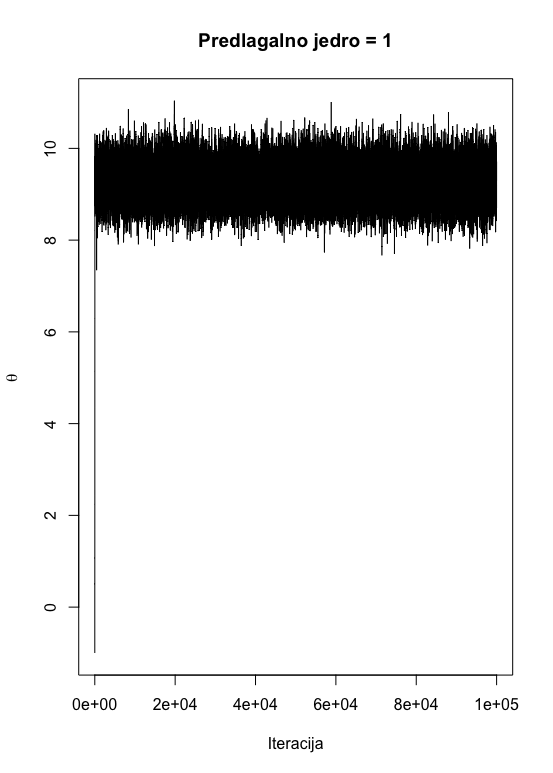
\includegraphics[width = 75mm]{Slike/4_1d_celotno.png}
            \caption{Celotno zaporedje.}
        \end{minipage}
    \end{figure}

    \begin{figure}[ht!]
        \begin{minipage}{0.5\textwidth}
            \centering
            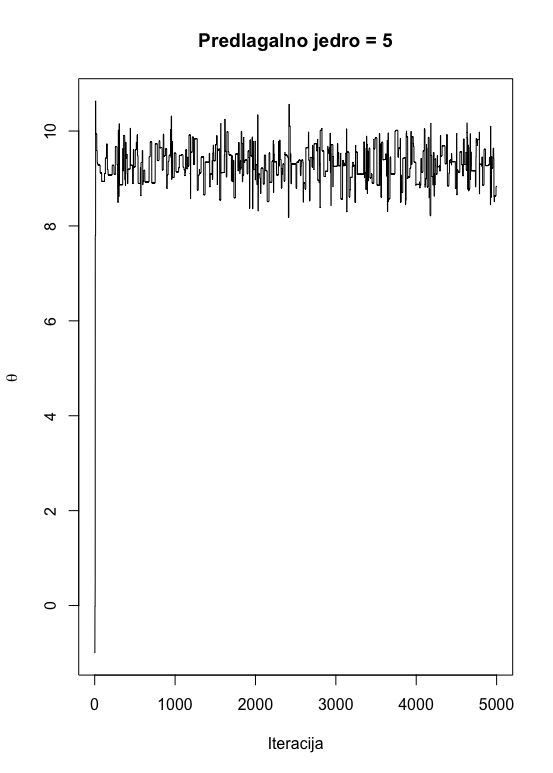
\includegraphics[width = 75mm]{Slike/4_1e_S.png}
            \caption{Prvih 5000 členov.}
        \end{minipage}
        \begin{minipage}{0.5\textwidth}
            \centering
            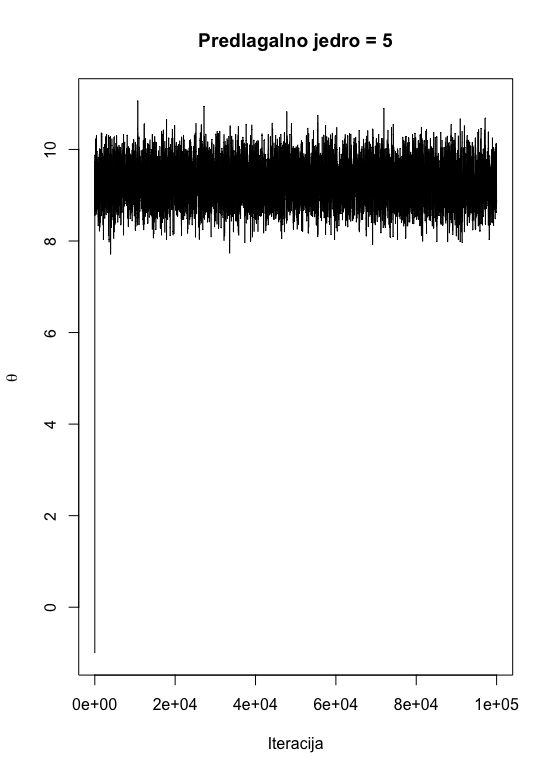
\includegraphics[width = 75mm]{Slike/4_1e_celotno.png}
            \caption{Celotno zaporedje.}
        \end{minipage}
    \end{figure}

    \begin{figure}[ht!]
        \begin{minipage}{0.5\textwidth}
            \centering
            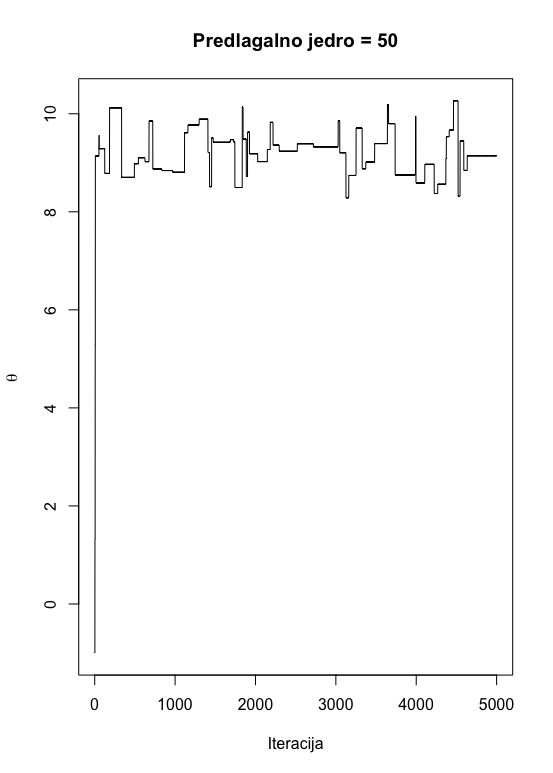
\includegraphics[width = 75mm]{Slike/4_1g_S.png}
            \caption{Prvih 5000 členov.}
        \end{minipage}
        \begin{minipage}{0.5\textwidth}
            \centering
            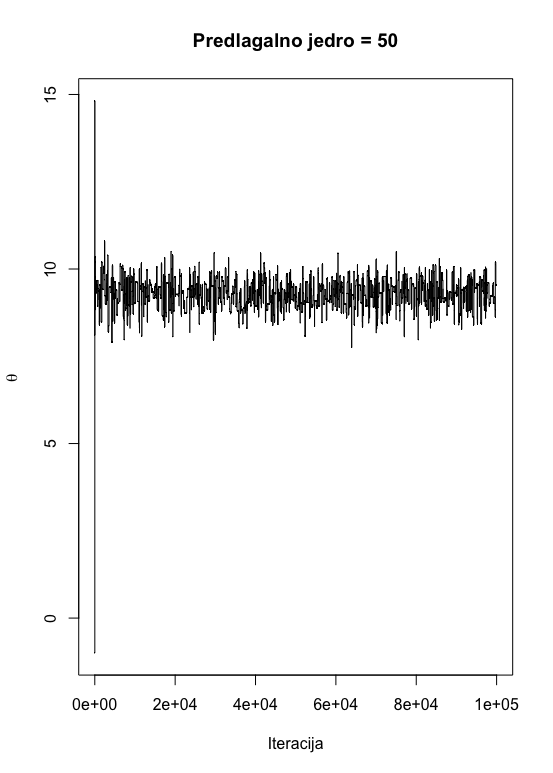
\includegraphics[width = 75mm]{Slike/4_1g_celotno.png}
            \caption{Celotno zaporedje.}
        \end{minipage}
    \end{figure}